\documentclass[aspectratio=169, table]{beamer}

\usepackage[utf8]{inputenc}
\usepackage{listings} 

\usetheme{Pradita}

\subtitle{MTI104 - IT Services}

\title{Session-01:\\\LARGE{Continual Improvement\\}}
\date[Serial]{\scriptsize {PRU/SPMI/FR-BM-18/0222}}
\author[Pradita]{\small{\textbf{Alfa Yohannis}}}

\begin{document}

\frame{\titlepage}

	
	\begin{frame}
		\frametitle{Lou Holtz's Quote}
		\begin{itemize}
			\item “In this world, you are either growing or you are dying.”
			\item Growth applies to all aspects of life: work, entertainment, and services.
			\item No product or service remains unchanged and rules the market for decades.
			\item Status quo leads to obsolescence.
			\item Constant enhancements are necessary for survival.
			\item Examples: Mobile phones, Internet service providers.
			\item ITIL's approach to continual improvement ensures ongoing value.
		\end{itemize}
	\end{frame}
	
	\begin{frame}
		\frametitle{Continual Improvement in SVS}
		\begin{itemize}
			\item Continual improvement is a key component of the Service Value System (SVS).
			\item It generates value and aligns with guiding principles.
			\item Improvements impact operational, tactical, and strategic levels.
			\item ITIL's continual improvement includes:
			\begin{itemize}
				\item Seven-step model
				\item Improve activity in SVC
				\item General practice for continual improvement
			\end{itemize}
		\end{itemize}
	\end{frame}
	
	\begin{frame}{Continual improvement in service value system}
	 \frametitle{Continual improvement in service value system}
\begin{center}
	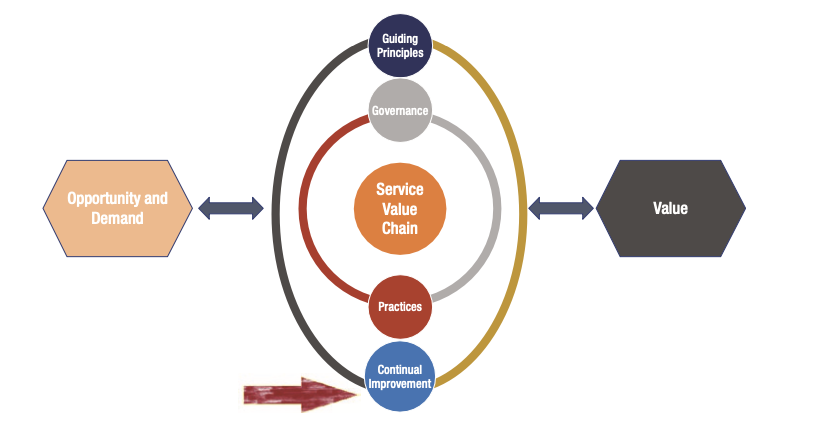
\includegraphics[width=0.8\linewidth]{images/image-01.png}
\end{center}
\end{frame}
	
	\begin{frame}
		\frametitle{Seven-Step Model}
		\begin{itemize}
			\item Originated in Lean, adapted in ITIL V3.
			\item Applied successfully across various domains.
			\item Logical steps that are iterative and adaptable.
			\item Aligns with organizational vision and mission.
			\item Steps include:
			\begin{itemize}
				\item Define what to improve
				\item Assess current state
				\item Set goals
				\item Identify improvement paths
				\item Implement changes
				\item Evaluate success
				\item Maintain momentum
			\end{itemize}
		\end{itemize}
	\end{frame}
	
	\begin{frame}
		\frametitle{Vision in Business}
		\begin{itemize}
			\item Vision sets long-term goals and objectives.
			\item Example: McDonald's real business as real estate.
			\item Understanding the customer’s vision is crucial.
			\item Align IT strategy with business vision and goals.
			\item Specific objectives are crucial for improvement.
			\item Improvement goals should be SMART:
			\begin{itemize}
				\item Specific
				\item Measurable
				\item Achievable
				\item Relevant
				\item Timebound
			\end{itemize}
		\end{itemize}
	\end{frame}
	
	\begin{frame}
		\frametitle{Where Are We Now?}
		\begin{itemize}
			\item Assess the current state to measure improvements.
			\item Conduct objective assessments of service aspects.
			\item Use measurements as a baseline for comparison.
			\item A baseline serves as a starting point.
			\item Missing this step impacts the accuracy of measuring improvements.
			\item Example: Performance improvements without baseline data.
		\end{itemize}
	\end{frame}
	
	\begin{frame}
		\frametitle{Where Do We Want to Be}
		\begin{itemize}
			\item Define specific, non-ambiguous goals.
			\item Perform gap analysis between current state and vision.
			\item Set Critical Success Factors (CSFs) and Key Performance Indicators (KPIs).
			\item Goals should follow the SMART principle.
			\item Goals should be specific and measurable.
			\item Example: Being the top burrito joint in the UK in 2 years.
		\end{itemize}
	\end{frame}
	
	\begin{frame}
		\frametitle{How Do We Get There?}
		\begin{itemize}
			\item Identify the best approach to achieve goals.
			\item Develop detailed plans and designs.
			\item Consider Agile or Waterfall methodologies as appropriate.
			\item Ensure alignment with overall vision.
			\item Managing risks and progress is crucial.
			\item Adapt to changing requirements as needed.
		\end{itemize}
	\end{frame}
	
	\begin{frame}
		\frametitle{Take Action}
		\begin{itemize}
			\item Implement changes based on the design.
			\item Adjust development approach as necessary.
			\item Manage typical project management aspects.
			\item Risk management and stakeholder engagement are key.
			\item Ensure improvements align with business needs.
			\item Monitor and adapt as required.
		\end{itemize}
	\end{frame}
	
	\begin{frame}
		\frametitle{Did We Get There?}
		\begin{itemize}
			\item Verify if the improvements meet objectives.
			\item Ensure the improvement is fit for use and purpose.
			\item Use iterative Agile methods to keep focus.
			\item Evaluate success or failure of the improvement.
			\item Maintain alignment with customer requirements.
			\item Validate and adjust as necessary.
		\end{itemize}
	\end{frame}
	
	\begin{frame}
		\frametitle{How Do We Keep the Momentum Going?}
		\begin{itemize}
			\item Continuous improvements are necessary.
			\item Encourage ongoing idea generation and innovation.
			\item Leadership and organizational culture play a role.
			\item Address failures and learn from them.
			\item Avoid stagnation and maintain focus on progress.
			\item Use failures as learning opportunities for future success.
		\end{itemize}
	\end{frame}
	
	\begin{frame}
		\frametitle{Continual Improvement Practice}
		\begin{itemize}
			\item Align practices with changing business needs.
			\item Identify and deliver improvements continuously.
			\item Foster a culture of improvement across the organization.
			\item Key activities include:
			\begin{itemize}
				\item Building a culture of improvement
				\item Idea registration and assessment
				\item Budget and resource allocation
				\item Project planning and delivery
				\item KPI measurement and evaluation
				\item Coordination and collaboration
			\end{itemize}
		\end{itemize}
	\end{frame}
	
	\begin{frame}
		\frametitle{Continual Improvement Tools}
		\begin{itemize}
			\item Continual Improvement Register (CIR)
			\item Improvement Reviews
			\item Development Methodology (Agile, Waterfall)
			\item Deployment Approach (Big Bang, Phase-wise)
			\item Use appropriate tools for effective improvement.
			\item Tools help in capturing, assessing, and implementing improvements.
		\end{itemize}
	\end{frame}
	
	\begin{frame}
		\frametitle{Engagement with Service Value Chain}
		\begin{itemize}
			\item Continual Improvement’s involvement in SVS:
			\begin{itemize}
				\item Planning: High involvement
				\item Design and Transition: High involvement
				\item Obtain/Build: High involvement
				\item Engage: Medium involvement
				\item Deliver and Support: High involvement
				\item Improve: High involvement
			\end{itemize}
			\item Improvement activities contribute to SVS effectiveness.
		\end{itemize}
	\end{frame}
	
	\begin{frame}
		\frametitle{Question}
		
		What is the importance of finding out where the organization is currently before embarking on identifying improvements?
		
		\begin{enumerate}[A.]
			\item A baseline serves as a starting point and as a comparison value for the progress made through improvements.
			\item Understanding where we are currently helps us understand the mistakes that were made earlier.
			\item It provides a balance in terms of the improvements that are taken before and after an improvement is delivered.
			\item The ground realities provide an excellent value to assess the relevance of improvement ideas.
		\end{enumerate}
		
	\end{frame}


\end{document}
